\documentclass[main.tex]{article}
\usepackage{subfiles}
\usepackage{hyperref}
\usepackage{csquotes}
\usepackage{amsmath}
\usepackage{amsfonts}
\usepackage[]{geometry}
\usepackage{graphicx}
\usepackage{listings}
\usepackage{xcolor}
\usepackage{subcaption}
\usepackage[section]{placeins}

\graphicspath{{./figures/}}

\begin{document}
    \section[P7: Random number experiment]{Experimenting sum of samples from Uniform Distribution}
    The result is demonstrated in Figure \ref{fig:p7-result} and code can be found in Appendix \ref{app:code-p7}.
    \par The experiment is to generate multiple random numbers from a \emph{Uniform Distribution} (0 to 1), sum them, store the result in a buffer and then do the same again. The resultant buffer has to be viewed as a normalized histogram.
    \par The resultant distribution achieved is called an \emph{Irwin-Hall distribution} which is defined as the sum of $n$ independent and identically distributed $U(0, 1)$ random variables.
    \begin{figure}[h]
        \centering
        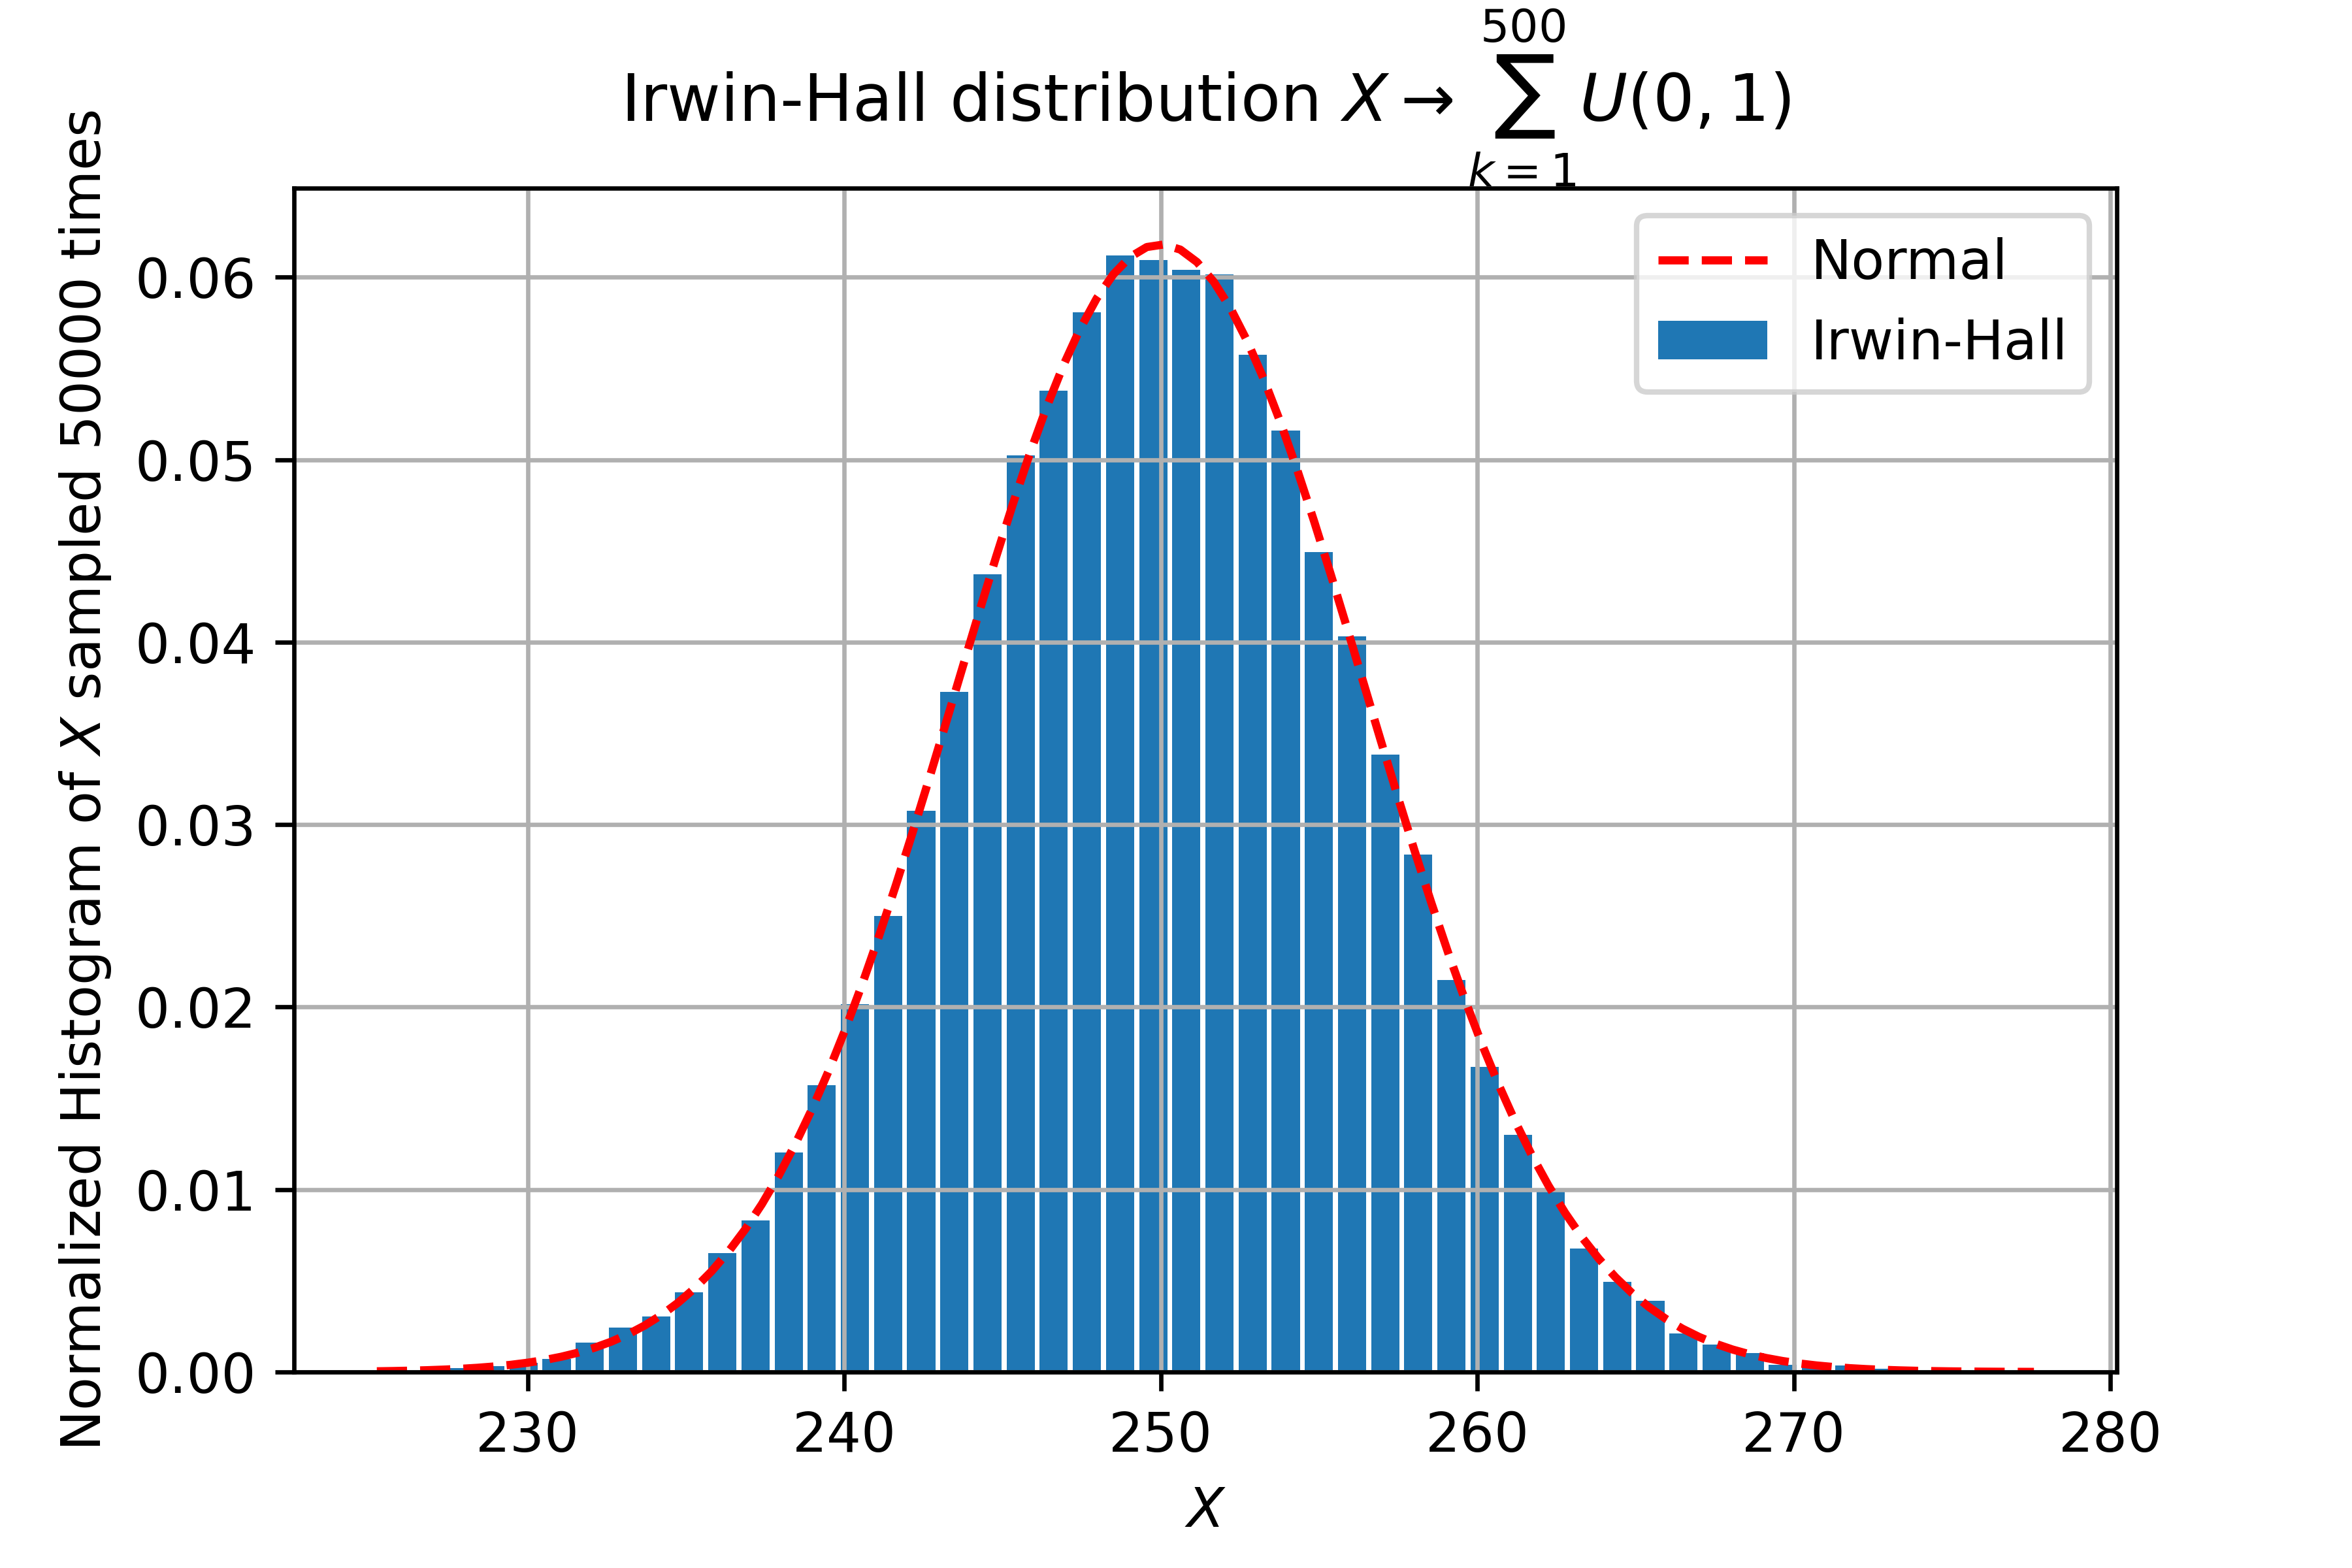
\includegraphics[width=0.9\textwidth]{plot_p7.png}
        \caption{Irwin-Hall Distribution}
        \label{fig:p7-result}
        \small This figure is obtained by visualizing the histogram of multiple experiments. In each experiment, 500 random numbers were generated from $U(0, 1)$ (uniform distribution) and added, the result being returned. The histogram is in blue, the red line is a \emph{normal distribution} with $\mu = \frac{N}{2} = 250$ and $\sigma^2 = \frac{N}{12} = 41.\bar{6}$. The code responsible for this figure can be found in Appendix A \ref{app:code-p7}.
    \end{figure}
    \subsection*{Irwin-Hall Distribution}
    The Irwin-Hall distribution is defined as the distribution of a continuous random variable $X$, where
    \begin{equation}
        X = \sum_{k=1}^{n} U(k; 0, 1)
    \end{equation}
    Basically, $X$ is the sum of $n$ independent and identically distributed uniform distributions (spanning 0 to 1). The probability density function is given by 
    \begin{equation}
        f_X(x; n) = \frac{1}{2\;(n-1)!} \sum_{k=0}^{n} (-1)^{k}
        \begin{pmatrix}
        n \\ 
        k
        \end{pmatrix}
        (x-k)^{n-1}\,\textup{sgn}(x-k)
    \end{equation}
    Where $\textup{sgn}$ is the sign function defined by
    \begin{equation}
        \textup{sgn}(x-k) = \left\{\begin{matrix}
            -1 & x < k \\
            0  & x = k \\
            +1 & x > k
            \end{matrix}\right.
    \end{equation}
    This is \textbf{different} from the normal distribution, but it can be \emph{approximated} to one by using $\mu = \frac{n}{2}$ and $\sigma^2 = \frac{n}{12}$ where $n$ is the number of times the summation is done. Such an approximated fit is shown in Figure \ref{fig:p7-result}.
\end{document}
